\chapter{狭义相对论}
%2019年 07月 24日 星期三 13:58:34 CST 
近几天研究狭义相对论,我的原始教材是郭硕鸿先生的《电动力学》(第二版),同时在学习过程中又参考过一些其它的教材.学习完成后总感觉理解的不是很到位,或者这也和工作繁忙没有时间集中时间研究有一定关系,但是我自己认为这个关系不大.在理论物理的学习过程中遇到了很多困难,经过努力逐步攻克了这些困难.最终我选择了朗道十卷作为我的主攻教材,这套书给了我很多逻辑清析,认识深刻的知识,对于相对论而言,朗道的论述是十分独到的.在此,我根据自己的学习理解,作了这一章的学习笔记.

\section{相互作用的传播速度}

\subsection{参考系}

描述自然界中所发生的现象需要有一个作为参考的物体,这个物体叫做\CJKunderwave{参考系}.在各种各样的参考系中有一个特殊的参考系,在此参考系中一个不受外力作用的物体将做匀速直线运动,这个参考系叫做\CJKunderwave{惯性参考系}.

\subsection{相对性原理}

\CJKunderwave{实验表明}所有的自然定律在所有惯性系中都是相同的.即表示自然定律的方程对于一个惯性系到另一个惯性系的时间与坐标的变换来说表达形式上是相同的.这个规律也是显然的,自然规律不应当与选择的参考系有关,唯一不同的可能是数值,但是函数关系应当是相同的.

\subsection{最大传播速度}

自然界中存在相互作用的两个物体,实验表明当其中一个物体发生任何变动时,仅仅只在某段时间以后才能被相互作用的另一个物体感知.我们以两个物体的距离除以从一个物体发生变动与另一个物体感知所用时间,得到相互作用的传播速度.当它们可以有多种方式相互作用时(比如同时有万有引力和电磁相互作用力),不同的作用有不同的传播速度.在某一参考系中我们可以找到一个最大的传播速度.当转换到另一个惯性系中时,这些传播速度会发生变化.但是我们不知道它是变大还是变小.假设两个惯性系A和B,在A中的最大传播速度为$v_{Amax}$,在B中的最大传播速度为$v_{Bmax}$,假设由A变换到B时,这个最大的传播速度变大了,则有$v_{Bmax}>v_{Amax}$,但是按照相对性原理从B变换到A时最大传播速度也应当变大了,所以得出$v_{Amax}>v_{Bmax}$显然二种情况是矛盾的,然而相对性原理是正确的,所以就得到在不同的惯性参考系中最大的传播速度必然相同.即$v_{Amax}=v_{Bmax}$,我们记此最大传播速度为$c$,则在所有的惯性系中它都是不变的.

从一个粒子向另一个粒子传播的相互作用往往又叫做``信号'',所以相互作用的传播速度又称为\CJKunderwave{信号速度}.这个最大的信号速度$c$就是光束,真空中的数值为
\begin{equation}
  c=2.998\times 10^8 m/s
  \label{eq:signalmax}
\end{equation}

\section{间隔}

在相对论中描述一个现象,我们需要指明它发生的地点和时间,这称为一个事件.即事件用一个四维坐标$(t,x,y,x)$来描述.在这个描述事件的四维空间中,一个事件对应到一组坐标,这组坐标称为四维空间中的一个点,因此我们可以说事件可以用点来表示,这个点叫做\CJKunderwave{世界点}.在假想的四维空间中,一个粒子对应若干个世界点,比如一个静止的粒子,在三维空间中它没有动,但是在四维空间中,它的时间坐标是一直增加的,由这些世界点连起来构成一条``曲线'',叫做\CJKunderwave{世界线}.一个做匀速直线运动的粒子,它各个坐标的比值都相同,所以可以说它的世界线是一条直线.一个做曲线运动的粒子,它的四维描述也是一系列的世界点,但是由于是曲线运动,则各坐标的比值不会是相同的,所以它的世界线也是曲线.

我们来研究光速在不同参考系中的测量.选定一个参考系$O$,在其中测量光速,事件1为光在此位置$(t_1,x_1,y_1,z_1)$发出,事件2为光在$(t_2,x_2,y_x,z_2)$接收.于是
\begin{equation}
c^2(t_2-t_1)^2-)(x_2-x_1)^2-(y_2-y_1)^2-(z_2-z_1)^2=0
  \label{eq:Olight0}
\end{equation}
选定第二个参考系$O'$,事件1为光在此位置$(t'_1,x'_1,y'_1,z'_1)$发出,事件2为光在$(t'_2,x'_2,y'_x,z'_2)$接收.于是
\begin{equation}
c^2(t'_2-t'_1)^2-)(x'_2-x'_1)^2-(y'_2-y'_1)^2-(z'_2-z'_1)^2=0
  \label{eq:Olight1}
\end{equation}
如果事件1和事件2不是以光速相联系,则上式必然就不等于零.同时由于光速是最大的信号速度,所以以上二式都应当大于等于零.记
\begin{equation}
  s_{12}=\sqrt{c^2(t_2-t_1)^2-(x_2-x_1)^2-(y_2-y_1)^2-(z_2-z_1)^2}
  \label{eq:jiange0}
\end{equation}
则$s_{12}$称为两个事件的间隔,显然有$s_{12}\geqslant 0$.为了讨论方便,我们取事件为在原点上,则间隔可以表达为
\begin{equation}
  s=\sqrt{c^2t^2-x^2-y^2-z^2}
  \label{eq:jiange}
\end{equation}

\subsection{朗道关于间隔不变性的论述}

下面讨论当坐标系变换后,间隔的变换规则.由于我们不知道$s^2$和$s'^2$的关系,所以我们可以假设其存在未知的函数关系,当$s^2$取微小变量$ds^2$时,则可以按$ds'^2$ Taylor展开.由于在测量光速中,当$s'^2=0$时$s^2=0$,所以展开的首项为0.则有下式成立
\begin{equation}
  ds^2=ads'^2
  \label{eq:jiange1}
\end{equation}
系数$a$ 只能与$O$和$O'$之间的相对运动的速度的大小有关.因为从$O$中的任何的一个世界点都可以做为起点,任何一个世界点都可以做为终点,只要二个世界点间的间隔相同,则在$O'$中也应当有相同的变换,这构成了惯性系的均匀性.如果$a$与速度的方向有关,则就与这里所述的惯性空间的均匀性相矛盾了.于是对于$O$和$O'$惯性系有
\begin{equation}
  ds^2=a(v_{1})ds'^2
  \label{eq:jiange2}
\end{equation}
同理对于$O$和$O''$惯性系有
\begin{equation}
  ds^2=a(v_{2})ds''^2
  \label{eq:jiange3}
\end{equation}
而对于$O'$和$O''$惯性系有
\begin{equation}
  ds'^2=a(v_{12})ds''^2
  \label{eq:jiange4}
\end{equation}
由式\eqref{eq:jiange2}和\eqref{eq:jiange3}联立可得
\begin{equation}
  ds'^2=\frac{a(v_{1})}{a(v_{2})}ds''^2
  \label{eq:jiange5}
\end{equation}
对比式\eqref{eq:jiange4}和式\eqref{eq:jiange5}可得
\begin{equation}
  a(v_{12})=\frac{a(v_{1})}{a(v_{2})}
  \label{eq:jiange6}
\end{equation}
在式\eqref{eq:jiange6}中左中含有$\vec{v}_1$和$\vec{v}_2$的夹角,但是在右式中不含有角度的信息,所以可以得到$a$只能是一个常数,所以由式\eqref{eq:jiange6}可得$a=1$.所以对于微小间隔满足
\begin{equation}
  ds^2=ds'^2
  \label{eq:jiange7}
\end{equation}
对于任何有限间隔,我们可以沿着世界线划分为若干无限小的间隔,则每一部分小间隔相等,再求和则可以得到对于有限间隔,在由一个惯性系换到另一个惯性系时也是不变的.即
\begin{equation}
  s^2=s'^2
  \label{eq:jiange8}
\end{equation}

\subsection{间隔不变性的第二种论述}

在$O$系二个事件的间隔满足关系(用$r^2=x^2+y^2+z^2$来简写)
\begin{equation}
  s^2=c^2t^2-r^2
  \label{eq:Jiange0}
\end{equation}
由相对性原理可得在$O'$系中考虑间隔的表达,也必然具备相同的函数结构,即
\begin{equation}
  s'^2=c^2t'^2-r'^2
  \label{eq:Jiange1}
\end{equation}
我们并不知道从$O$到$O'$中,坐标是如何变化的,则不防可以假设一个未知的函数关系,考虑每个$O$中的坐标用$O'$中各坐标表示的函数的Taylor级数,则由于相对性原理的限制,则可知这个函数关系必然只能具有线性项.同时能变换成相同的结构,则二个间隔必然具有关系
\begin{equation}
  s^2=As'^2
  \label{eq:Jiange2}
\end{equation}
我们再考虑一个惯性系$O''$,则从$O$到$O''$的变换可以有两种情况.其一,从$O$到$O'$再到$O''$得到
\begin{equation}
  s^2=As'^2=A^2s''^2
  \label{eq:Jiange3}
\end{equation}
其二,从$O$直接到$O''$则得到
\begin{equation}
  s^2=As''^2
  \label{eq:Jiange4}
\end{equation}
对照式\eqref{eq:Jiange3}和式\eqref{eq:Jiange4}可得
\begin{gather}
  A^2=A
  \intertext{解得}
  A=1
  \intertext{所以可得间隔不变}
  s^2=s'^2
\end{gather}

\section{洛仑兹变换}

这一节讨论洛仑兹变换的三种不同导出方式.先来论证一下,与运动方向垂直的坐标不发生变换.如图\ref{fig:lorentz0}所示.

\begin{figure}[H]
  \centering
  \begin{tikzpicture}
    \draw[pattern=north east lines] (-0.5,2.2)--++(0,-0.2)--++(1,0)--++(0,0.2);
    \draw[pattern=north east lines] (-0.5,-0.2)--++(0,0.2)--++(1,0)--++(0,-0.2);
    \draw (0,-0.2) node [anchor=north]{\small $M$};
    \draw (0,2.2) node [anchor=south]{\small $N$};
    \draw[->,>=stealth] (-0.2,0)--(-0.2,2);
    \draw[<-,>=stealth] (0.2,0)--(0.2,2);
    \draw (-0.2,1) node [anchor=east]{\small $z'$};
  \end{tikzpicture}
  \qquad
  \begin{tikzpicture}
    \draw[pattern=north east lines] (-2,-0.2)--++(0,0.2)--++(1,0)--++(0,-0.2);
    \draw[pattern=north east lines] (1,-0.2)--++(0,0.2)--++(1,0)--++(0,-0.2);
    \draw[pattern=north east lines] (-0.5,2.2)--++(0,-0.2)--++(1,0)--++(0,0.2);
    \draw[->,>=stealth] (-1.5,0)--(0,2);
    \draw[<-,>=stealth] (1.5,0)--(0,2);
    \draw[->,>=stealth] (-1.5,0)--(1.5,0);
    \draw[dashed](0,0)--(0,2);
    \draw (-1,1) node [anchor=east] {\small $\frac{c\Delta t}{2}$};
    \draw (0,0) node [anchor=north]{\small $v\Delta t$};
    \draw (-1.5,-0.2) node [anchor=north]{\small $M$};
    \draw (1.5,-0.2) node [anchor=north]{\small $M$};
    \draw (0,2.2) node [anchor=south]{\small $N$};
    \draw (0,1) node [anchor=west]{\small $z$};
  \end{tikzpicture}
  \caption{垂直分量不变}
  \label{fig:lorentz0}
\end{figure}

考虑光从$M$发出事件到从$N$反回最后再从$M$接收事件.则图\ref{fig:lorentz0}所示左侧为和$M$因联的惯性系中观察到的现象.则
\begin{equation}
  s'^2=c^2(\Delta t')^2=4z'^2
  \label{eq:lorentz0}
\end{equation}
在$O$惯性系中,有
\begin{equation}
  s^2=c^2(\Delta t)^2 -v^2(\Delta t)^2=4z^2
  \label{eq:lorentz1}
\end{equation}
由间隔不变原理,据式\eqref{eq:lorentz0}和式\eqref{eq:lorentz1}可得
\begin{equation}
  z'=z
  \label{eq:lorentz2}
\end{equation}
即:与运动方向垂直的分量不发生变化.

\subsection{方案一}

将洛仑兹变换写为
\begin{gather}
  \left\{
    \begin{gathered}
      x'=a_{11}x+a_{12}ct\\
      ct'=a_{21}x+a_{22}ct
    \end{gathered}
  \right.
\end{gather}
  计算间隔
\begin{align}
  s^2&=c^2t'^2-x'^2\notag\\
  &=(a_{22}^2-a_{12}^2)c^2t^2-(a_{11}^2-a_{12}^2)x^2\notag\\
  &+2(a_{21}a_{22}-a_{11}a_{12})ct\cdot x
\end{align}
于是间隔不变性要求:
\begin{gather}
  \left\{
    \begin{gathered}
      a_{22}^2-a_{12}^2=1\\ 
      a_{11}^2-a_{21}^2=1\\ 
      a_{21}a_{22}-a_{11}a_{12}=0
    \end{gathered}
  \right.
  \label{eq:lorentz3}
\end{gather}
由式\eqref{eq:lorentz3}可得
\begin{equation}
  \frac{a_{21}}{a_{11}}=\frac{a_{12}}{a_{22}}
  \label{eq:lorentz4}
\end{equation}
同时,由于当速度远小于光速时相对论应当回归到经典力学,所以可以判断$a_{11}>0$和$a_{22}>0$,则
\begin{equation}
  a_{11}=\sqrt{1+a_{12}^2}\qquad a_{22}=\sqrt{1+a_{12}^2}
  \label{eq:lorentz5}
\end{equation}
由式\eqref{eq:lorentz4}和式\eqref{eq:lorentz5}对比可得:$a_{12}=a_{21}$.在$O$系中追踪$O'$的运动,则
\begin{gather}
  0=a_{11}vt+a_{12}ct\notag\\
  \intertext{推出}
  \frac{a_{12}}{a_{11}}=-\frac{v}{c}\notag
  \intertext{代入式\eqref{eq:lorentz5}得}
  \left\{
    \begin{gathered}
      a_{11}=\frac{1}{\sqrt{1-\frac{v^2}{c^2}}}\\
      a_{12}=\frac{-v/c}{\sqrt{1-\frac{v^2}{c^2}}}\\
    \end{gathered}
  \right.
  \intertext{于是得到洛仑兹变换}
  \left\{
    \begin{gathered}
      x'=\frac{x-vt}{\sqrt{1-\frac{v^2}{c^2}}}\\
      t'=\frac{t-\frac{v}{c^2}x}{\sqrt{1-\frac{v^2}{c^2}}}
    \end{gathered}
  \right.
\end{gather}

\subsection{方案二}

此推证方法源于一次在期中考试监考过程中偶然想到的.将洛仑兹变换写为

\begin{gather}
  \left\{
    \begin{gathered}
      x'=a_{11}x+a_{12}ct\\
      ct'=a_{21}x+a_{22}ct
    \end{gathered}
  \right.
\end{gather}
追踪$O'$相对于$O$的运动,则
\begin{gather}
  0=a_{11}vt+a_{12}ct
  \intertext{解得}
  \frac{a_{12}}{a_{11}}=-\frac{v}{c}
\end{gather}
将上式代入洛仑兹变换第一式,得
\begin{equation}
  x'=a_{11}(x-vt)
  \label{eq:lorentz6}
\end{equation}
基于相对性原理,可得逆变换
\begin{equation}
  x=a_{11}(x'+vt')
  \label{eq:lorentz7}
\end{equation}
由式\eqref{eq:lorentz6}考虑光传播这一事实,则
\begin{gather}
  ct'=a_{11}(c-v)t
  \intertext{解得}
  \frac{t'}{t}=a_{11}(1-\frac{v}{c})
  \label{eq:lorentz8}
\end{gather}
同理,由式\eqref{eq:lorentz7}考虑光传播这一事实,则
\begin{gather}
  ct=a_{11}(c+v)t'
  \intertext{解得}
  \frac{t'}{t}=\frac{1}{a_{11}}{1+\frac{v}{c}}
  \label{eq:lorentz9}
\end{gather}
式\eqref{eq:lorentz8}和式\eqref{eq:lorentz9}相等,则
\begin{gather}
  a_{11}(1-\frac{v}{c})=\frac{1}{a_{11}(1+\frac{v}{c})}
  \intertext{解得}
  a_{11}=\frac{1}{\sqrt{1-\frac{v^2}{c^2}}}
  \label{eq:lorentz10}
\end{gather}
将式\eqref{eq:lorentz10}代入式\eqref{eq:lorentz6}和式\eqref{eq:lorentz7}联立二式得洛仑兹变换为
\begin{gather}
  \left\{
    \begin{gathered}
      x'=\frac{x-vt}{\sqrt{1-\frac{v^2}{c^2}}}\\
      t'=\frac{t-\frac{v}{c^2}x}{\sqrt{1-\frac{v^2}{c^2}}}
    \end{gathered}
  \right.
\end{gather}

\subsection{方案三}

此法源自于朗道的《场论》 \S4 .二事件的间隔可以认为是在四维空间内的相对应的世界点的距离.所求变换要对距离保持不变,所以在数学上对应四维坐标(ct,x,y,z)的转动.四维空间内的一切转动可以化为六个分别在平面 xy,zy,xz,tx,ty,tz内的转动,考虑到一个特例---在tx平面内的转动.则需借助双曲函数完成,已知双曲函数满足关系
\begin{gather}
\cosh^2\theta-\sinh^2\theta=1
\intertext{所以tx平面内的转动为}
 \left\{
   \begin{gathered}
    x=x'\cosh\theta +ct'\sinh\theta\\
    ct=x'\sinh\theta+ct'\cosh\theta
   \end{gathered}
 \right.
 \label{eq:lorentz11}
\intertext{追踪$O'$在$O$系中的运动,$x'=0$则}
 \left\{
   \begin{gathered}
    vt=ct'\sinh\theta\\
    ct=ct'\cosh\theta
   \end{gathered}
 \right.
 \intertext{解得}
 \tanh\theta=\frac{v}{c}
 \intertext{由于$\cosh\theta>0$所以有}
 \left\{
   \begin{gathered}
     \cosh\theta=\frac{1}{\sqrt{1-\tanh^2\theta}}=\frac{1}{\sqrt{1-\frac{v^2}{c^2}}}\\
     \sinh\theta=\cosh\theta\tanh\theta=\frac{\frac{v}{c}}{\sqrt{1-\frac{v^2}{c^2}}}
   \end{gathered}
 \right.
 \label{eq:lorentz12}
 \intertext{式\eqref{eq:lorentz12}代入式\eqref{eq:lorentz11}得洛仑兹变换}
 \left\{
   \begin{gathered}
     x=\frac{x'+vt'}{\sqrt{1-\frac{v^2}{c^2}}}\\
     t=\frac{t'+\frac{v}{c^2}x'}{\sqrt{1-\frac{v^2}{c^2}}}
   \end{gathered}
 \right.
   \qquad
 \left\{
   \begin{gathered}
     x'=\frac{x-vt}{\sqrt{1-\frac{v^2}{c^2}}}\\
     t'=\frac{t-\frac{v}{c^2}x}{\sqrt{1-\frac{v^2}{c^2}}}
   \end{gathered}
 \right.
 \label{eq:lorentz13}
\end{gather}

\section{固有时}

对比洛仑兹变换和伽利略变换,则它们有很大的不同.原因在于伽利略变换默认的是信号速度是无限大的,所以当物体的速度远小于光速时洛仑兹变换将退回到伽利略变换.这个变化将导致描述物体的运动时对于时间和空间的记录问题,有相应的变更.在伽利略变换中,由于时间是绝对的,它不依赖于任何参考系.所以在经典力学中,记录时间可以在任何位置的时钟上读出数值.但是在相对论中这样做是不行的!我们可以看到,对于一个运动的物体,使其本身携带一个时钟,则可以在这个时钟确定此物体经历的时间.下面来详细讨论这个描述运动的计时问题.

在惯性系$O$中,我们固定在原点$O$上一时钟,当物体在原点时我们可以由此读出时刻.当物体运动另一点时再来读取这个时钟所指示的时刻时就有问题,由于信号速度是有限的,当光由原点传到物体所在地点时物体将会发生运动而到达了另一个位置.所以这是不可行.处理这个问题的关键是在任何一个地点处放置一个与原点的钟对过时的钟,当物体来到此处时就在此处读取时钟的时刻,则这个时刻就是原点处时钟所指示的读数.由于相对论效应,又产生了如何对准时钟的问题.由于当物体运动的速度远小于光速时,坐标间的变换将回到伽利略变换,则时间将变成绝对的.所以可以首先将所有的完全相同的时钟放置在原点$O$处,对齐示数,然后以无限缓慢的速度移动到空间的每一个位置上.这样在空间的每一点上就有一个和原点指示计数相同的钟.这样我们就和经典的情况不相矛盾了,当物体由$A$移动到$B$时,分别从$A$和$B$读取时刻,相减后得到经历的时间.由于各个时钟是和原点时钟对过时的,所以\CJKunderwave{可以认为运动所需要的时间就是原点时钟所指示的时间},只是读取方式上的不同而己.在运动的参考系$O'$原点处也固定一个时钟,由于它在运动,所以它指示的时间和$O$系中是不一样的,但是在$O'$系中,我们也用同样的方法在每一点安放了时钟的,它们所指示的时间和$O'$处的钟示数是相同的.

由上述讨论可知,每一个惯性系,其原点处的时钟决定了整个坐标系的时间问题.因此,原点处的钟指示的时刻我们称为固有时.一个运动的物体,在原点$O'$的钟指示的数值就是此参考系的固有时.

下面我们来讨论$O$系和$O'$中的固有时的关系. 和$O'$中任一位置$x'$固定的时钟,它指示的时间总是在$x'$时的值,但是由于在$O$看来,$O'$是运动的,则在$O$中经历的时间将是由$O$中不同的位置(即$O'$)所在处的时钟指示的时刻计算出来的,由于对过时,所以它也就是$O$处不动时钟的示数.基于这个关系,考虑洛仑兹变换式
\begin{gather}
  \left\{
    \begin{gathered}
      t_1=\frac{t_1'+\frac{v}{c^2}x'}{\sqrt{1-\frac{v^2}{c^2}}}\\
      t_2=\frac{t_2'+\frac{v}{c^2}x'}{\sqrt{1-\frac{v^2}{c^2}}}
    \end{gathered}
  \right.
  \label{eq:guyoushi0}
  \intertext{注意$x_1\neq x_2$ ,所以令二者相减得}
  \Delta t =\frac{\Delta t'}{\sqrt{1-\frac{v^2}{c^2}}}
\end{gather}
由上述讨论可得$\Delta t >\Delta t'$ 即一物体运动起来后,其上的固有时$\Delta t'$和其静止于$O$系时的固有时$\Delta t$ 相比变小了,即运动物体的时钟变慢了!

讨论完时间,我们再来讨论一下距离.当一个刚性杆,注意是刚性的!它不能发生实质性的变形.在此杆在$O$中沿$x$轴匀速直线运动时,我们要测量它的长度,必须在同一时刻测定!这可以通过在杆的两端上放上两个人在同一时刻$t$读取在$O$中的坐标,然后相减我们就得到了它的长度.但是在和杆固连的$O'$系中,由于杆是静止的,所以测量它两端的坐标不受时间限制,所以在$O'$中测量杆的长度时,可以先在$t'_1$时读取$A$端坐标$x'_A$,然后跑到另一端,时间必定不与之相同了,即在$t'_2$时刻读取$B$端坐标$x'_B$,则在$O'$中杆的长度为$\Delta x'=x'_B-x'_A$.由于在$O'$中讨论杆的长度对时刻没有限制,所以考虑逆洛仑兹变换式
\begin{gather}
  \left\{
    \begin{gathered}
      x'_1=\frac{x_1-vt}{\sqrt{1-\frac{v^2}{c^2}}}\\
      x'_2=\frac{x_2-vt}{\sqrt{1-\frac{v^2}{c^2}}}
    \end{gathered}
  \right.
  \label{eq:guyoushi1}
  \intertext{注意$t'_1\neq t'_2$ ,所以令二者相减得}
  \Delta x'=\frac{\Delta x}{\sqrt{1-\frac{v^2}{c^2}}}
  \intertext{简单计算可得}
  \Delta x=\Delta x'\cdot\sqrt{1-\frac{v^2}{c^2}}
\end{gather}
由上述可得,一个不可伸缩的刚性杆,由于相对论效应会导致在标静止时的长度和运动起来时的长度有所不同.即在$O$系中测得运动杆长$\Delta x$和$O'$系中测得的静止杆长$\Delta x'$相比要小!即运动的刚性杆变短了!


\section{相对论的速度变换}

如果一个物体在$O$和$O'$中都是运动的,则它们的速度变换关系叫做相对论的速度变换.借助洛仑兹变换不难得到这一变换.
\begin{gather}
 \left\{
   \begin{gathered}
     t=\frac{t'+\frac{v}{c^2}x'}{\sqrt{1-\frac{v^2}{c^2}}}\\
     x=\frac{x'+vt'}{\sqrt{1-\frac{v^2}{c^2}}}\\
     y=y'\\
     z=z'
   \end{gathered}
 \right.
 \label{eq:vtransform0}
 \intertext{分别取微小变量,得}
 \left\{
   \begin{gathered}
     \Delta t=\frac{1+\frac{vu'_x}{c^2}}{\sqrt{1-\frac{v^2}{c^2}}}\Delta t'\\
     \Delta x=\frac{u'_x+v}{\sqrt{1-\frac{v^2}{c^2}}}\Delta t'\\
     \Delta y =\Delta y'\\
     \Delta z=\Delta z'
   \end{gathered}
 \right.
 \label{eq:vtransform1}
 \intertext{令式\eqref{eq:vtransform1}中后三式除以第一式的时间,可得}
 \left\{
   \begin{gathered}
     u_x=\frac{u'_x+v}{1+\frac{vu'_x}{c^2}}\\
     u_y=\frac{u'_y\sqrt{1-\frac{v^2}{c^2}}}{1+\frac{u'_xv}{c^2}}\\
     u_z=\frac{u'_z\sqrt{1-\frac{v^2}{c^2}}}{1+\frac{u'_xv}{c^2}}
   \end{gathered}
 \right.
\end{gather}

\section{相对论中的力学量}

\subsection{自由粒子的拉格朗日函数}

自由粒子在惯性系中做匀速直线运动.同时由欧几里德几何可知三维空间中两点间直线最短,所以对于四维空间中的间隔就对应有一个结论,从一个世界点到另一个世界点,积分$\int \mathrm{d}s$沿直世界线进行时,具有最大值.原因在于,对于两个确定的世界点,则它们之间的时间是确定的,但是三维空间中的路径可以有多种,而当路径为直线时$r^2$最小,由间隔的定义$s^2=c^2t^2-r^2$可得,当路径为直线时间隔是最大的.对于一个自由粒子而言,它的实际路径就是直线,所以其沿世界线的积分$\int \mathrm{d}s$将具备最大值.

按照分析力学中的最小作用原理,主函数的变分具有最小值.综合自由粒子沿世界线的积分最大,而主函数又是一个标量所以其应当为洛仑兹不变量,同时在洛仑兹变换中又有间隔不变原理,据此可以推断出自由粒子主函数一定具备如下形式
\begin{equation}
  S=-\alpha \int \mathrm{d}s
  \label{eq:zhuhanshuS}
\end{equation}
式中$\alpha$是一个大于零的实数.下面来确定常数$\alpha$的值,将间隔用固有时表出,则
\begin{equation}
  S=-\alpha c \int \mathrm{d}\tau =-\alpha c \int \sqrt{1-\frac{v^2}{c^2}} \mathrm{d}t
  \label{eq:zhuhanshuS0}
\end{equation}
式\eqref{eq:zhuhanshuS0}和主函数的定义对比可得拉格朗日函数为
\begin{equation}
  L=-\alpha c \sqrt{1-\frac{v^2}{c^2}}
  \label{eq:zhuhanshuS1}
\end{equation}
当$v \ll c$时,相对论的公式应当回归到经典情况,将式\eqref{eq:zhuhanshuS1}Taylor 展开,然后取$v^2$项得
\begin{equation}
  L=-\alpha c -\frac{1}{2}\alpha \frac{v^2}{c}
  \label{eq:zhuhanshuS2}
\end{equation}
同时经典的情况为
\begin{equation}
  L=\frac{1}{2}mv^2
  \label{eq:zhuhanshuS3}
\end{equation}
由于在拉格朗日函数中多一个常数不会有任何影响,所以对比式\eqref{eq:zhuhanshuS2}和式\eqref{eq:zhuhanshuS3}可得常数$\alpha =  mc$.于是相对论中的拉格朗日函数为
\begin{equation}
  L=-mc^2\sqrt{1-\frac{v^2}{c^2}}
  \label{eq:zhuhanshuS4}
\end{equation}
由分析力学可知
\begin{equation}
  p_i =-\frac{\partial S}{\partial x^i}=\frac{\partial L}{\partial v^i}
  \label{eq:zhuhanshuS5}
\end{equation}
由于主函数作为一个标量,其梯度是一个洛仑兹协变矢量,所以可以由式\eqref{eq:zhuhanshuS5}求出四维动量(其满足洛仑兹协变性)为
\begin{equation}
  p_i=\left (\frac{E}{c},-\frac{m\vec{v}}{\sqrt{1-\frac{v^2}{c^2}}}\right )
  \label{eq:zhuhanshuS6}
\end{equation}
所以可得在相对论中的动量表达式为
\begin{equation}
  \vec{p}=\frac{m\vec{v}}{\sqrt{1-\frac{v^2}{c^2}}}
  \label{eq:zhuhanshuS10}
\end{equation}
显然当$v\ll c$时,式\eqref{eq:zhuhanshuS10}回归到经典公式$\vec{p}=m\vec{v}$.同理可以得到四维动量的逆变形式为
\begin{equation}
  p^i=\left (\frac{E}{c},\frac{m\vec{v}}{\sqrt{1-\frac{v^2}{c^2}}}\right )
  =\left(\frac{E}{c},\vec{p}\right)
  \label{eq:zhuhanshuS11}
\end{equation}
考虑到动量与速度的经典关系,所以可以得出四维速度的表达式(此处兼顾了朗道书的定义)
\begin{equation}
  u^i=\frac{p^i}{mc}=\left(\frac{E}{mc^2},\frac{\vec{v}}{c\sqrt{1-\frac{v^2}{c^2}}}\right)
  \label{eq:zhuhanshuS12}
\end{equation}
在式\eqref{eq:zhuhanshuS12}中的速度部分,显然其是坐标对间隔的微分,即
\begin{equation}
  \frac{\mathrm{d}\vec{r}}{\mathrm{d}s}=\frac{\vec{v}}{c\sqrt{1-\frac{v^2}{c^2}}}
  \label{eq:zhuhanshuS13}
\end{equation}
而四维坐标的表达式为
\begin{equation}
  x^i=\left( ct,\vec{r}\right)
  \label{eq:zhuhanshuS14}
\end{equation}
四维坐标是协变矢量,间隔为洛仑兹不变量,所以一个协变矢量对一个洛仑兹不变量微分也将获得一个洛仑兹矢量.即
\begin{equation}
  u^i=\frac{\mathrm{d}x^i}{\mathrm{d}s}=\left(\frac{1}{\sqrt{1-\frac{v^2}{c^2}}},\frac{\vec{v}}{c\sqrt{1-\frac{v^2}{c^2}}}\right)
  \label{eq:zhuhanshuS15}
\end{equation}
对照式\eqref{eq:zhuhanshuS15}和式\eqref{eq:zhuhanshuS12}的第零分量,可得相对论下自由粒子的能量为
\begin{equation}
  E=\frac{mc^2}{\sqrt{1-\frac{v^2}{c^2}}}
  \label{eq:zhuhanshuS16}
\end{equation}
于是四维动量又可以写作
\begin{equation}
  p^i=\left (\frac{mc}{\sqrt{1-\frac{v^2}{c^2}}},\frac{m\vec{v}}{\sqrt{1-\frac{v^2}{c^2}}}\right )
  \label{eq:zhuhanshuS17}
\end{equation}
由内积的变换不变性,考虑式\eqref{eq:zhuhanshuS11}和式\eqref{eq:zhuhanshuS17},由于变换不变性,则在式\eqref{eq:zhuhanshuS17}中取$v=0$也不影响内积,则可得能量与动量的相对论关系为
\begin{gather}
  p^ip_i=\frac{E^2}{c^2}-p^2=m^2c^2
  \intertext{所以相对论能量与动量的关系为}
  \frac{E^2}{c^2}=p^2+m^2c^2
  \label{eq:zhuhanshuS18}
\end{gather}
由四维动量的定义,同时考虑内积的洛仑兹不变性可得
\begin{gather}
  p^ip_i=m^2c^2
  \intertext{上式对间隔微分可得}
  p^i\frac{\mathrm{d}p_i}{\mathrm{d}s}=0
  \intertext{经过简单计算得}
  \frac{mc}{\sqrt{1-\frac{v^2}{c^2}}}\cdot\frac{\mathrm{d}p^0}{\mathrm{d}{s}}
  -\frac{m\vec{v}\cdot\vec{f}}{c(1-\frac{v^2}{c^2})}=0
  \intertext{由此可以方便得到动量第零分量对间隔的微分}
  \frac{\mathrm{d}p^0}{\mathrm{d}s}
  =\frac{\vec{f}\cdot\vec{v}}{c^2\sqrt{1-\frac{v^2}{c^2}}}
  \intertext{于是得四维力为}
  g^i=\frac{\mathrm{d}p^i}{\mathrm{d}s}=
  \left(
    \frac{\vec{f}\cdot\vec{v}}{c^2\sqrt{1-\frac{v^2}{c^2}}},
  \frac{\vec{f}}{c\sqrt{1-\frac{v^2}{c^2}}}
  \right)
\end{gather}
上式中力$\vec{f}=\frac{\mathrm{d}\vec{p}}{\mathrm{d}t}$,仍然是动量对时间的导数.

\subsection{再议速度变换公式}

上一节定出了四维速度的形式,在$O$系中即
\begin{equation}
  u^i=\frac{\mathrm{d}}{\mathrm{d}s}\left(ct,\vec{r}\right)
  \label{eq:4weiV}
\end{equation}
上述间隔在随物体一块运动的参考系中表出,同时为了书写简洁选择速度单位为光速$c$,则
\begin{equation}
  u^i=\left(\frac{1}{\sqrt{1-u_x^2}},\frac{\vec{u}}{\sqrt{1-u_x^2}}\right)
  \label{eq:4weiV0}
\end{equation}
同理在$O'$系中表出物体的四维坐标,除以该物体在随其自身一同运动的参考系中的间隔表达式,则
\begin{equation}
  u'^i=\left(\frac{1}{\sqrt{1-u^{\prime 2}}_x},\frac{\vec{u}'}{\sqrt{1-u^{\prime 2}_x}}\right)
  \label{eq:4weiV1}
\end{equation}
四维速度满足洛仑兹变换,注意在洛仑兹变换中的速度$v$是$O'$相对于$O$运动的速度.则
\begin{gather}
  \left\{
    \begin{gathered}
      \frac{u_x}{\sqrt{1-u_x^2}}=\frac{u'_x+v}{\sqrt{1-u^{\prime 2}_x}\sqrt{1-v^2}}\\ 
      \frac{u_y}{\sqrt{1-u_x^2}}=\frac{u_y'}{\sqrt{1-u^{\prime 2}_x}}\\
      \frac{u_z}{\sqrt{1-u_x^2}}=\frac{u_z'}{\sqrt{1-u^{\prime 2}_x}}\\
      \frac{1}{\sqrt{1-u_x^2}}=\frac{1+u'_xv}{\sqrt{1-u^{\prime 2}_x}\sqrt{1-v^2}}
    \end{gathered}
  \right.
  \label{eq:4weiV2}
  \intertext{由式\eqref{eq:4weiV1}中前三式分另除以第四式可得速度变换关系为}
  \left\{
    \begin{gathered}
      u_x=\frac{u'_x+v}{1+u'_xv}\\
      u_y=\frac{u'_y\sqrt{1-v^2}}{1+u'_xv}\\
      u_z=\frac{u'_z\sqrt{1-v^2}}{1+u'_xv}
    \end{gathered}
  \right.
  \label{eq:4weiV3}
  \intertext{如果恢复为国际单位,则式\eqref{eq:4weiV3}化为}
 \left\{
   \begin{gathered}
     u_x=\frac{u'_x+v}{1+\frac{vu'_x}{c^2}}\\
     u_y=\frac{u'_y\sqrt{1-\frac{v^2}{c^2}}}{1+\frac{u'_xv}{c^2}}\\
     u_z=\frac{u'_z\sqrt{1-\frac{v^2}{c^2}}}{1+\frac{u'_xv}{c^2}}
   \end{gathered}
 \right.
\end{gather}

\section{相对速度}

\subsection{不变量标量计算法}

在$O$系中有两个物体1和2,其速度分别为$\vec{v}_1$和$\vec{v}_2$,考虑内积的洛仑兹不变性,为了方便书写,以光速$c$作为速度的单位,则相当于所有公式中令$c=1$即可,于是
\begin{gather}
  p_{1i}p^{2i}=\frac{m_1m_2}{\sqrt{1-v^2}}
  \label{eq:xiangduiV}
  \intertext{上式右式是在认为2的速度为零时的相对坐标系中写出的,左式在$O$系中写出,则}
  \frac{m_1m_2}{\sqrt{(1-v_1^2)(1-v_2^2)}}-m_1m_2v_1v_2\cos\theta=\frac{m_1m_2}{\sqrt{1-v^2}}
  \intertext{上式约去$m_1m_2$,经过简单计算可得}
  v=\frac{\sqrt{v_1^2+v_2^2-2v_1v_2\cos\theta +v_1^2v_2^2\sin^2\theta}}{1-v_1v_2\cos\theta}
  \intertext{上式也可以写为更加简洁的矢量式}
  v=\frac{\sqrt{(\vec{v}_1-\vec{v}_2)^2-(\vec{v}_1\times\vec{v}_2)^2}}{1-\vec{v}_1\cdot\vec{v}_2}
\end{gather}
显然,当物体的速度远小于光速时,即$v_1\ll 1,v_2\ll 1$时,上式化经典情况
\begin{equation}
  v=\left|\vec{v}_1-\vec{v}_2\right|
  \label{eq:xiangduiV0}
\end{equation}

\subsection{矢量计算法}

在$O_0$中物体1和2的速度分别为$\vec{v}_1$和$\vec{v}_2$,此处隐含着还有一个物体参与运动,也就是参考系$O_0$,要求出2相对于1的相对速度,必须假定1不动,此时需确定$O_0$相对于1的速度也就是$-\vec{v}_1$.而此时2相对于$O_0$的速度还是$\vec{v}_2$,实际上这里的问题转化为三步:第一步,求出$O_0$相对于1的速度,而1变成了参考系$O$,原来的$O_0$变成了$O'$.第二步,物体2相对于$O_0$的运动,现在变成是在新的$O'$中的运动,其速度仍然为$\vec{v}_2$.第三步,由洛仑兹变换求出新$O$系中物体2的速度,也就是2相对于1的速度了.

为了讨论问题的方便仍然取速度单位为光速,同时取$\vec{v}_1$方向为$x$轴.则$O'$相对于$O$的速度为$-v_1$,由洛仑兹变换得2相对于1的速度$\vec{v}$为
\begin{gather}
\left\{
  \begin{gathered}
    v_x=\frac{v_{2x}-v_1}{1-v_{2x}v_1}\\
    v_y=\frac{v_y\sqrt{1-v_1^2}}{1-v_{2x}v_1}\\
    v_z=\frac{v_z\sqrt{1-v_1^2}}{1-v_{2x}v_1}
  \end{gathered}
\right.
\end{gather}
下面求相对速度的大小
\begin{align}
  v&=\sqrt{v_x^2+v_y^2+v_z^2}\notag\\
  &=\frac{\sqrt{(v_{2x}-v_1)^2+v_{2y}^2(1-v_1^2)+v_{2z}^2(1-v_1)^2}}{1-v_{2x}v_1}\notag\\
  &=\frac{\sqrt{v_1^2+v_2^2-2v_{2x}v_1-(v_{2y}^2+v_{2z}^2)v_1^2}}{1-v_{2x}v_1}\notag
  \intertext{上式可以写成矢量式,如此则与所确定的坐标轴指向就没有特定的关系了,于是得}
  &=\frac{\sqrt{(\vec{v}_1-\vec{v}_2)^2-(\vec{v}_1\times\vec{v}_2)^2}}{1-\vec{v}_1\cdot\vec{v}_2}
  \label{eq:xiangduiV1}
\end{align}

\section{分布函数的变化}

\subsection{基本数学原理}

在这一节谈到了动量``体积元''的变换,用到了超曲面等概念,我对此并不是很熟悉,所以在此消耗了较长的时间来说明这一问题.考虑一个n+1维矢量
\begin{equation}
  A=(a_1,a_2,\cdots,a_{n+1})
\end{equation}
我们来确定与A垂直的n+1维矢量的最大个数,以$B_i$表示第$i$个与A垂直的矢量.则这个问题转化为了下列方程组最多有几个非零解的问题.按照克莱姆法则求线性代数解的方法易知,与A垂直的n+1维向量最多只能有n个,即
\begin{gather}
  \left\{
    \begin{gathered}
      a_1b_{11}+a_2b_{12}+\cdots a_{n+1}b_{1,n+1}=0\notag\\
      a_1b_{21}+a_2b_{22}+\cdots a_{n+1}b_{2,n+1}=0\notag\\
      \cdots  \notag\\
      a_1b_{n1}+a_2b_{n2}+\cdots a_{n+1}b_{n,n+1}=0\notag
    \end{gathered}
  \right.
  \label{eq:NweiS0}
\end{gather}
同时按照行列式的计算规则,如果有两行(或两列)相同,则行列式的值为零.以$\vec{e}_i$表示n+1维向量的各个基,也就是说A的实体表示为
\begin{equation}
  A=a_1\vec{e}_1+a_2\vec{e}_2+\cdots+a_{n+1}\vec{e}_{n+1}
  \label{eq:NweiS1}
\end{equation}
如下用实体基构建行列式
\begin{equation}
  C=
  \begin{vmatrix}
    \vec{e}_1&\vec{e}_2&\vec{e}_3&\cdots&\vec{e}_{n+1}\\
    b_{11}&b_{12}&b_{13}&\cdots&b_{1,n+1}\\
    b_{21}&b_{22}&b_{23}&\cdots&b_{2,n+1}\\
    &&\vdots&&\\
    b_{n1}&b_{n2}&b_{n3}&\cdots&b_{n,n+1}
  \end{vmatrix}
\end{equation}
显然考虑$B_i$与C的内积,相当于以第i个B矢量的各个分量分别取代C第一行的n+1个基,原因是n+1个基是相互正交的.显然B的这n个矢量都与C垂直.同时在n+1维空间内与C垂直的矢量必然都线性相关.于是可得C与A是线性相关的.设比例系数为$\lambda$,下面我们来说明在线性变换下此系数是不变的.设变换矩阵为D,则
\begin{gather}
  C=\lambda A
  \intertext{以D分别左作用上式得}
  CD=\lambda AD
  \intertext{由于$C'=CD$,$A'=AD$,所以在新的基底下有}
  C'=\lambda A' 
\end{gather}
这就说明了,如果两个高维向量线性相关,则在线性变换它们的比例系数是不变的.同时,因为比例系数是一个标量,所以它是不变的也不难理解.

\subsection{动量微元的变换}

在相对论中动量的内积是一个洛仑兹不变量.于是我们可以得到一个垂直关系,即
\begin{gather}
  p^ip_i=m^2c^2
  \intertext{对上式取变分,则}
  p^i\delta p_i=0
\end{gather}
$p^i$是一个四维矢量,所以能够找到的线性无关的与$p^i$垂直的三个四维矢量.一个最简单的取法是当取$\mathrm{d}p_x$时,其余动量变化都是零,但是能量会有相应的变化,于是这样的三个四维矢量分别可以取为
\begin{gather}
  \left\{
    \begin{gathered}
      \left(\mathrm{d}E_1,\mathrm{d}p_x,0,0\right)\\ 
      \left(\mathrm{d}E_1,0,\mathrm{d}p_y,0\right)\\ 
      \left(\mathrm{d}E_1,0,0,\mathrm{d}p_z\right)
    \end{gathered}
  \right.
\end{gather}
于是考虑由这三个矢量构成的外积,则必然与四维矢量$p^i$线性相关,则比例系数是一个洛仑兹不变量.即这个外积是
\begin{equation}
  \begin{vmatrix}
    \vec{e}_0 & \vec{e}_1&\vec{e}_2&\vec{e}_3\\
    \mathrm{d}E_1&\mathrm{d}p_x&0&0\\
    \mathrm{d}E_2&0&\mathrm{d}p_y&0\\
    \mathrm{d}E_3&0&0&\mathrm{d}p_z
  \end{vmatrix}
  \label{eq:dongliangP}
\end{equation}
显然外积第零分量为$\mathrm{d}p_x\mathrm{d}p_y\mathrm{d}p_z$,四维动量$p^i$的第零分量为$E$,所以其比例系数$\lambda$为
\begin{equation}
  \lambda =\frac{\mathrm{d}p_x\mathrm{d}p_y\mathrm{d}p_z}{E}
  \label{eq:dongliangP1}
\end{equation}
根据前述的高维微量分析可知,在洛仑兹变换过程中比例系数是不发生变化的.

粒子数$f\mathrm{d}p_x\mathrm{d}p_y\mathrm{d}p_z$是一个标量,显然它不应当随参考系的变换而发生变化,将其写为
\begin{equation}
  f(\vec{p})\mathrm{d}p_x\mathrm{d}p_y\mathrm{d}p_z
  =
  f(\vec{p})E\frac{\mathrm{d}p_x\mathrm{d}p_y\mathrm{d}p_z}{E}
  \label{eq:dongliangP2}
\end{equation}
则分布函数与能量的乘积是一个不变量.则
\begin{equation}
  f(\vec{p})E=f(\vec{p}^{\ \prime})E'
  \label{eq:dongliangP3}
\end{equation}

同时由于动量和能量的关系$E^2=p^2+m^2$,所以可得$p\mathrm{d}p=E\mathrm{d}E$,于是将动量微元写成球坐标的形式,得
\begin{equation}
  \frac{\mathrm{d}p_x\mathrm{d}p_y\mathrm{d}p_z}{E}=
  \frac{p^2\mathrm{d}p\mathrm{d}o}{E}=p\mathrm{d}E\mathrm{d}o
  \label{eq:dongliangP4}
\end{equation}
于是又得到一个不变量$p\mathrm{d}E\mathrm{d}o$.对于体积,由洛仑兹变换可得

\begin{gather}
  \mathrm{d}V=\mathrm{d}V_0\sqrt{1-v^2}\qquad
  \mathrm{d}V'=\mathrm{d}V_0\sqrt{1-v^{\prime2}}
  \intertext{所以有}
  \frac{\mathrm{d}V}{\mathrm{d}V'}=
  \frac{\sqrt{1-v^2}}{\sqrt{1-v^{\prime2}}}
  =\frac{E'}{E}
  =\frac{\mathrm{d}p'_x\mathrm{d}p'_y\mathrm{d}p'_z}{\mathrm{d}p_x\mathrm{d}p_y\mathrm{d}p_z}
  \intertext{所以可得}
\mathrm{d}V\mathrm{d}p_x\mathrm{d}p_y\mathrm{d}p_z=
\mathrm{d}V'\mathrm{d}p'_x\mathrm{d}p'_y\mathrm{d}p'_z
\end{gather}
于是可得相空间内的体元$\mathrm{d}\tau$也是一个洛仑兹不变量.同时由于在一个相元内的粒子数$f\mathrm{d}\tau$显然也是一个不变量,所以可得分布函数$f(\vec{r},\vec{p})$也是一个不变量.

\section{粒子的衰变}

这一节的讨论的内容不难,但是在习题中分析衰变后粒子的最大偏角时的计算其实有点麻烦.在这里首先引一个我在高中时期分析出的椭圆计算公式,在此处可以极大的降低计算量.

\subsection{椭圆的解析分析}

如图所示
\begin{figure}[H]
  \centering
  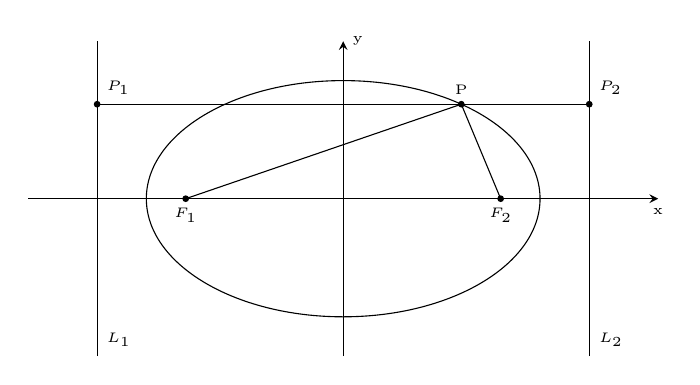
\begin{tikzpicture}
    \draw [->,>=stealth](-4,0)--(4,0) node [anchor=north]{\tiny x};
    \draw [->,>=stealth](0,-2)--(0,2) node [anchor=west]{\tiny y};
    \filldraw (2,0) circle [radius=1pt] node [anchor=north]{\tiny $F_2$};
    \filldraw (-2,0) circle [radius=1pt] node [anchor=north]{\tiny $F_1$};
    \draw(-3.125,-2)--(-3.125,2);
    \draw(3.125,-2)--(3.125,2);
    \draw (0,0) ellipse (2.5 and 1.5);
    \draw (-2,0)--(1.5,1.2)--(2,0);
    \filldraw (1.5,1.2) circle [radius=1pt] node [anchor=south]{\tiny P};
    \draw (-3.125,1.2)--(3.125,1.2);
    \filldraw (-3.125,1.2) circle [radius=1pt] node [anchor=south west] {\tiny $P_1$};
    \filldraw (3.125,1.2) circle [radius=1pt] node [anchor=south west] {\tiny $P_2$};
    \draw (-3.125,-2)node [anchor=south west] {\tiny $L_1$};
    \draw (3.125,-2)node [anchor=south west] {\tiny $L_2$};
  \end{tikzpicture}
  \caption{椭圆}
  \label{fig:tuoyuan}
\end{figure}

\begin{gather}
  \intertext{椭圆的标准解析方程为} 
  \frac{x^2}{a^2}+\frac{y^2}{b^2}=1
  \label{eq:tuoyuan}
  \intertext{准线方程为}
  \left\{
    \begin{gathered}
      l_1:x_1=-\frac{a^2}{c}\\
      l_2:x_2=\frac{a^2}{c}
    \end{gathered}
  \right.
  \intertext{定和性质:}
  |PF_1|+|PF_2|=2a
  \intertext{定比性质:}
  \frac{|PF_1|}{|PP_1|}=\frac{|PF_2|}{|PP_2|}=e=\frac{c}{a}
  \intertext{e为离心率.过椭圆上一点$(x_0,y_0)$的切线方程:}
  \frac{xx_0}{a^2}+\frac{yy_0}{b^2}=1
  \intertext{记斜率为k,则切线的斜率和切点间的关系为}
  k\cdot\frac{y_0}{x_0}=-\frac{b^2}{a^2}
  \intertext{一般高中常用联立方程的形式求$x_1+x_2$,$y_1+y_2$,$x_1x_2$,$y_1y_2$.高考中数学大题必出此类型,从对称的观点可以证明下式成立.}
  \left\{
    \begin{gathered}
      \frac{x^2}{a^2}+\frac{y^2}{b^2}=1\\
      Ax+By+C=0 
    \end{gathered}
  \right.
  \intertext{由直线解得$y=-\frac{Ax+C}{B}$代入椭圆方程可得}
  (A^2a^2+B^2b^2)x^2+Aa^22Cx+a^2(C^2-B^2b^2)=0
  \intertext{注意上式是极其对称的,为了快速解题,需要同学位根据对称的特点背过.其判别式为}
  \Delta_x=4a^2b^2B^2(A^2a^2+B^2b^2-C^2)
  \intertext{于是判定直线与椭圆有无交点只需判断$A^2a^2+B^2b^2$与$C^2$的大小关系即可.}
  A^2a^2+B^2b^2>C^2
  \intertext{上式成立则有两个交点}
  A^2a^2+B^2b^2=C^2
  \intertext{上式成立则有一个交点}
  A^2a^2+B^2b^2<C^2
  \intertext{上式成立则无交点,同时基于x,y的同等地位和对称性,易写出关于y的联立方程式和判别式}
  \left\{
    \begin{gathered}
      (A^2a^2+B^2b^2)y^2+Bb^22Cy+b^2(C^2-A^2a^2)=0\\
      \Delta_y=4a^2b^2A^2(A^2a^2+B^2b^2-C^2)
    \end{gathered}
  \right.
  \intertext{显然由韦达定理易得$x_1+x_2$,$y_1+y_2$,$x_1x_2$,$y_1y-2$之值,此不再赘述.下面再来看一看弦长的问题.一般的x方程为:}
  (x-x_1)(x-x_2)=0\notag\\
  x^2-(x_1+x_2)x+x_1x_2=0\notag\\
  \Delta_x=(x_1+x_2)^2-4x_1x_2=(x_1-x_2)^2
  \intertext{同理}
  \Delta_y=(y_1-y_2)^2
  \intertext{所以有弦长l为}
  l=\sqrt{(x_1-x_2)^2+(y_1-y_2)^2}=\sqrt{\Delta_x+\Delta_y}\notag
  \intertext{代入$\Delta_x$和$\Delta_y$解得}
  l=\frac{2ab}{A^2a^2+B^2b^2}\sqrt{(A^2+B^2)(A^2a^2+B^2b^2-C^2)}
\end{gather}

\subsection{衰变时粒子的偏角问题}

此问题源于习题的第1题:一个以速度V运动的粒子在``飞行''中分解为两个粒子.求这些粒子的出射角同其能量的能量间的关系.

在此问题中可以认为这个飞行的粒子本来就由两个粒子构成,两个粒子以共同的速度V飞行,在某一时刻分离开来,而具体结节则由二者相互作用决定.取其中一个粒子其在C系中的能量为$E_0$,在L系中能量为$E$,出射角为在L系中观察的,所以由洛仑兹变换得
\begin{equation}
  E_0=\frac{E-Vp\cos\theta}{\sqrt{1-V^2}}
  \label{eq:shuaibian}
\end{equation}
解得
\begin{equation}
  \cos\theta =\frac{E-E_0\sqrt{1-V^2}}{Vp}
  \label{eq:shuaibian0}
\end{equation}
同时考虑到动量和能量关系,则$p=\sqrt{E^2-m^2}$代入上式得
\begin{equation}
  \cos\theta =\frac{E-E_0\sqrt{1-V^2}}{V\sqrt{E^2-m^2}}
  \label{eq:shuaibian1}
\end{equation}

对偏转角的范围在动量变换中分析比较容易.在发生衰变的平面内可以取为xy平面,则衰变前后动量的z分量都为0.在动量中心系C中研究问题较方便,在此系中两个粒子初始都处于静止状态,衰变后则两个以相同动量大小向相反的两个方向飞去(由于动量守恒,则二个粒子动量大小相同),设在C系中加以下标``0'',则由洛仑兹变换得
\begin{gather}
  \left\{
    \begin{gathered}
      p_x=\frac{p_{x0}+E_0V}{\sqrt{1-V^2}}\\
      p_y=p_{y0}
    \end{gathered}
  \right.
\end{gather}
至于在C系中,具体的能量和动量取为何值这取决于衰变的性质,而仅有的数据不能确定.所以写出$p_x,p_y$的关系,得
\begin{gather}
  \frac{\left(p_x-\frac{VE_0}{1-V^2}\right)^2}{\left(p_0/\sqrt{1-V^2}\right)}
  +\frac{p_y^2}{p_0^2}=1
\end{gather}
当$\frac{VE_0}{\sqrt{1-V^2}}<p_0/\sqrt{1-V^2}$时,原点位于椭圆内部,则此时夹角为$\theta$的可能性只有一种.当$\frac{VE_0}{\sqrt{1-V^2}}>p_0/\sqrt{1-V^2}$时,则原点位于椭圆外部,则对应于一个$\theta$角,有两个可能的动量值.但是这个角有一定的限度,当过原点的直线与椭圆相切时此角达到最大.写出直线方程为
\begin{equation}
\tan\theta_m \cdot (p_x-\frac{VE_0}{1-V^2})-p_y+\tan\theta_m\frac{VE_0}{1-V^2}
=0
  \label{eq:shuaibian2}
\end{equation}
由椭圆与直线相切的条件$A^2a^2+B^2b^2=C^2$可得
\begin{gather}
  \tan^2\theta_m\cdot\frac{p_0^2}{1-V^2}+p_0^2=\tan^2\theta_m\cdot\frac{V^2E_0^2}{1-V^2} 
  \intertext{将$E_0^2=p_0^2+m^2$代入上式得}
  \tan^2\theta_m\cdot\frac{p_0^2}{1-V^2}+p_0^2=\tan^2\theta_m\cdot\frac{V^2(p_0^2+m^2)}{1-V^2} 
  \intertext{简单计算可得 }
  \sin\theta_m=\frac{p_0\sqrt{1-V^2}}{mV}
\end{gather}

在{\bf\S13 粒子的弹性碰撞}一节,式13.8也有和此处类似的推证,下面说明之.二个粒子1和2发生弹性碰撞,则L系中始情况为2静止,1以速度$\vec{v_1}$运动.所发生的弹性碰撞过程可以理解为开始二者的动量不同,在相互作用的过程中必然有一个时刻二者以共同的速度运动,由于整个过程中动量守恒所以这个速度就是动量中心系的速度V.下一个时刻二都分离,则1以一定的角度射出,从达到共同速度之后的过程可以等价于一个以速度V运动着的复合粒子发生发衰变.所以这和衰变的分析是相同的.唯一要做的是求出质心速度V.下面的计算中,认为``衰变''过程中分析的是第一个粒子,则
\begin{gather}
  \vec{p}=\vec{p}_1\notag\\
  E=E_1+m_2\notag
  \intertext{所以质心的速度为}
  V=\frac{\vec{p}}{E}=\frac{\vec{p}_1}{E_1+m_2}
\end{gather}
2粒子初始时在L系中静止,所以相对于质心的速度大小也为$V$,于是在C系中2的初始动量为
\begin{equation}
  \frac{m_2V}{\sqrt{1-V^2}}
\end{equation}
由于发生的是弹性碰撞,则在C系来看仅仅是粒子的速度方向发生了变化,其动量大小没有变化.所以``衰变''后2粒子的动量与初始的值大小相同.由于在质心系中总动量为零,所以1在衰变后的动量也与2的动量数值相同.所以得到
\begin{equation}
 p_0=\frac{m_2V}{\sqrt{1-V^2}}
\end{equation}
解得
\begin{equation}
  m_2=\frac{p_0\sqrt{1-V^2}}{V}
  \label{eq:shuaibian3}
\end{equation}
所以存在最大角的条件$\frac{VE_0}{\sqrt{1-V^2}}>p_0/\sqrt{1-V^2}$变为
\begin{gather}
  VE_0>p_0
  \intertext{将能量用1的质量表达出来,$p_0$ 用2的质量表达出来}
  \frac{Vm_1}{\sqrt{1-V^2}}>\frac{m_2V}{\sqrt{1-V^2}}
  \intertext{即}
  m_1>m_2
\end{gather}
此时的最大角$\theta_m$为
\begin{gather}
  \sin\theta_m=\frac{p_0\sqrt{1-V^2}}{m_1V}=\frac{m_2}{m_1}
\end{gather}
